\documentclass[dvipdfmx]{jsarticle}
%\documentclass[a4j]{ujarticle}
\usepackage{resume}  % resume用スタイル
\usepackage{udline}  % 下線用
\usepackage{comment} % 複数行コメント

\pagestyle{plain}

\begin{document}
\twocolumn[
    \beginheader{令和5年度 コンピュータサイエンス研究II 中間審査会}{2023}{8}{8}{井上研究室}
    \title{TravelatAR : 地表面近似テクスチャーのアニメーション重畳表示よる\\歩行速度制御システム}
    \affiliation{東京工科大学大学院 バイオ・情報メディア研究科 コンピュータサイエンス専攻}
    \author{G2122014 島谷~~優佑}
    \endheader
]

\vspace{3mm}
%\setcounter{page}{1}

%------------------------------------------------------------------
\section{はじめに}
人間の歩行運動は歩行の向きと速度の2つに分けて考えることができる.
歩行の向きを外部から操作することで人々の目的地を誘導することができる.
歩行速度を外部から操作することができれば,空間の混雑緩和や健康維持への効果が期待できるため,
社会的な需要が高い.
これまで,歩行速度は路面や標識に印字された記号や文字,警備員による音声案内によって誘導をしてきた.
しかし,これらは混雑の具合によっては歩行者が認識できないことも多い他,
音声ガイドによる指示の強制力は必ずしも高くない.
このような背景から,記号や音声ではなく,幾何学的な視覚刺激を用いて歩行速度を操作する研究が実施されている.
%------------------------------------------------------------------

谷崎らは実空間を歩行中の被験者にヘッドマウントディスプレイを通してオプティカルフローの速度と中心視野を変化させたバーチャル空間を提示し,
被験者の歩行速度の変化を調べた\cite{article2}.
その結果,オプティカルフローの速度と被験者の歩行速度の間に負の相関があることが示唆された.
この手法は VRに基づいており,現実空間の歩行速度誘導に利用するのは難しい.


櫻木らはARグラスを通して見える床面上に「動く歩道」のテクスチャをアニメーション提示し,
その際の被験者の歩行運動を観察した\cite{article1}.
この手法はARに基づいており,現実空間の歩行速度誘導への適合性が高いものの,
著者らが期待した誘導効果は確認できなかった.
その理由として,ARで提示したテクスチャの見た目が現実の床面の見た目と差があること,
歩行の際にテクスチャの隙間から床面が見えてしまい,ユーザからみた現実感
(ユーザから見える空間の整合性?)が低下したことの影響を挙げている.
%------------------------------------------------------------------

本研究ではARを用いた行動制御方法では床に現実にを模していないバーチャル床をアニメーション重畳表示して見せるより,
現実の床を模したバーチャル床をアニメーション重畳表示した方が没入感が高まり,
ユーザの動きをより制御できると考える.
本稿では芝生道にて,芝生を模したバーチャル床を表示した場合,
芝生を模していないバーチャル床を表示した場合に比べてユーザの歩行速度制御に
優位性が出るか否かの調査を行う.
%------------------------------------------------------------------
\section{TravelatAR}
本研究ではユーザの視界に映る床に現実の床を模したバーチャル床をアニメーション重畳表示するシステムを提案する.


\subsection{システム概要}
図\ref{fig:gaiyo}に本システムの概要を示す.
本システムでは被験者にARグラスを装着してもらう.
これにより,現実の床を模したバーチャル床ををユーザの視界にアニメーション表示する.
\begin{figure}[t]
    \centering
    \fbox{
    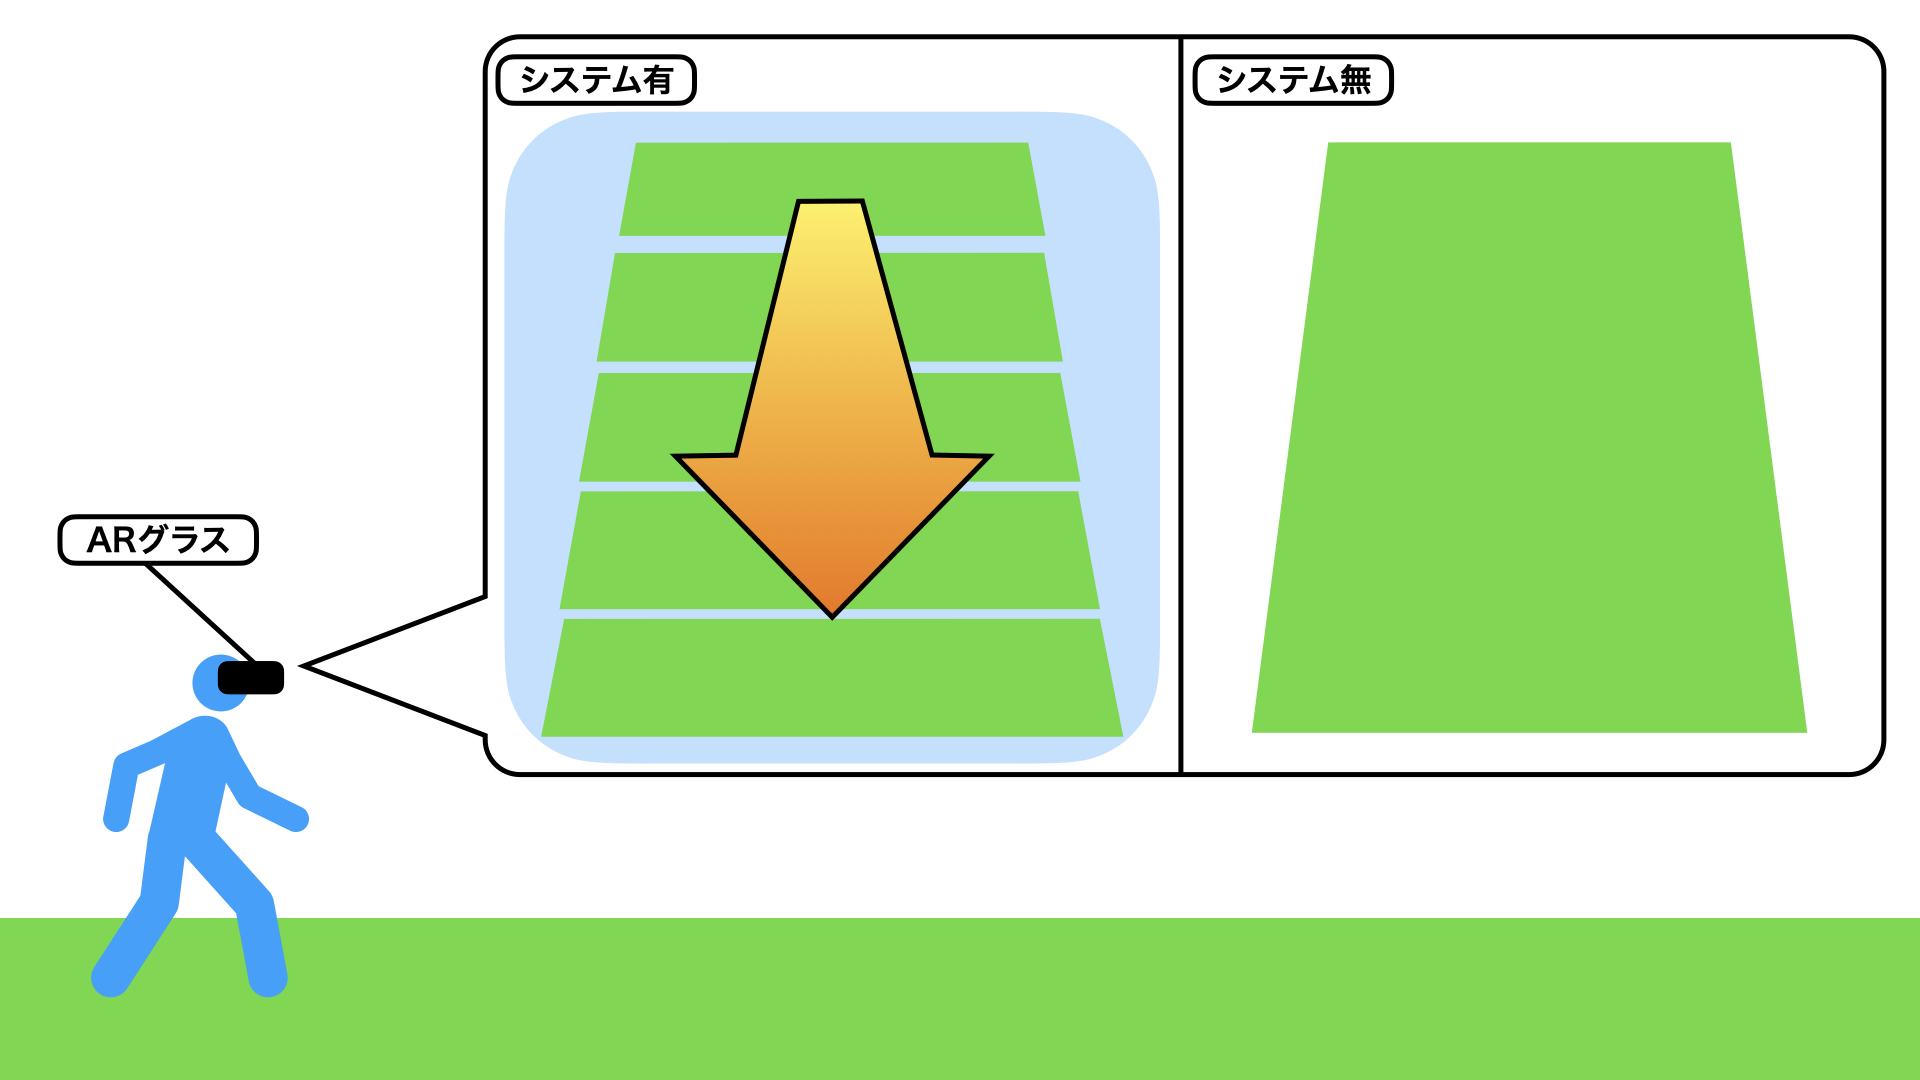
\includegraphics[width=1.1\linewidth]{fig/gaiyo.001.jpeg}
    }
    \caption{システム概要図}
    \label{fig:gaiyo}
\end{figure}

\subsection{リアルテクスチャ}
ユーザが歩く道の地表面に近似したテクスチャを作成する.
本システムでは,これらのテクスチャをバーチャル床にアタッチし被験者の視界の床にアニメーション重畳表示を行う.
本稿では人工芝の道を歩くことを想定したリアルテクスチャ作成した.
また,リアルテクスチャの比較対象となる地表面に近似していないNonリアルテクスチャを複数作成した.
\subsection{プロトタイプ}
\begin{figure}[t]
    \centering
    \fbox{
    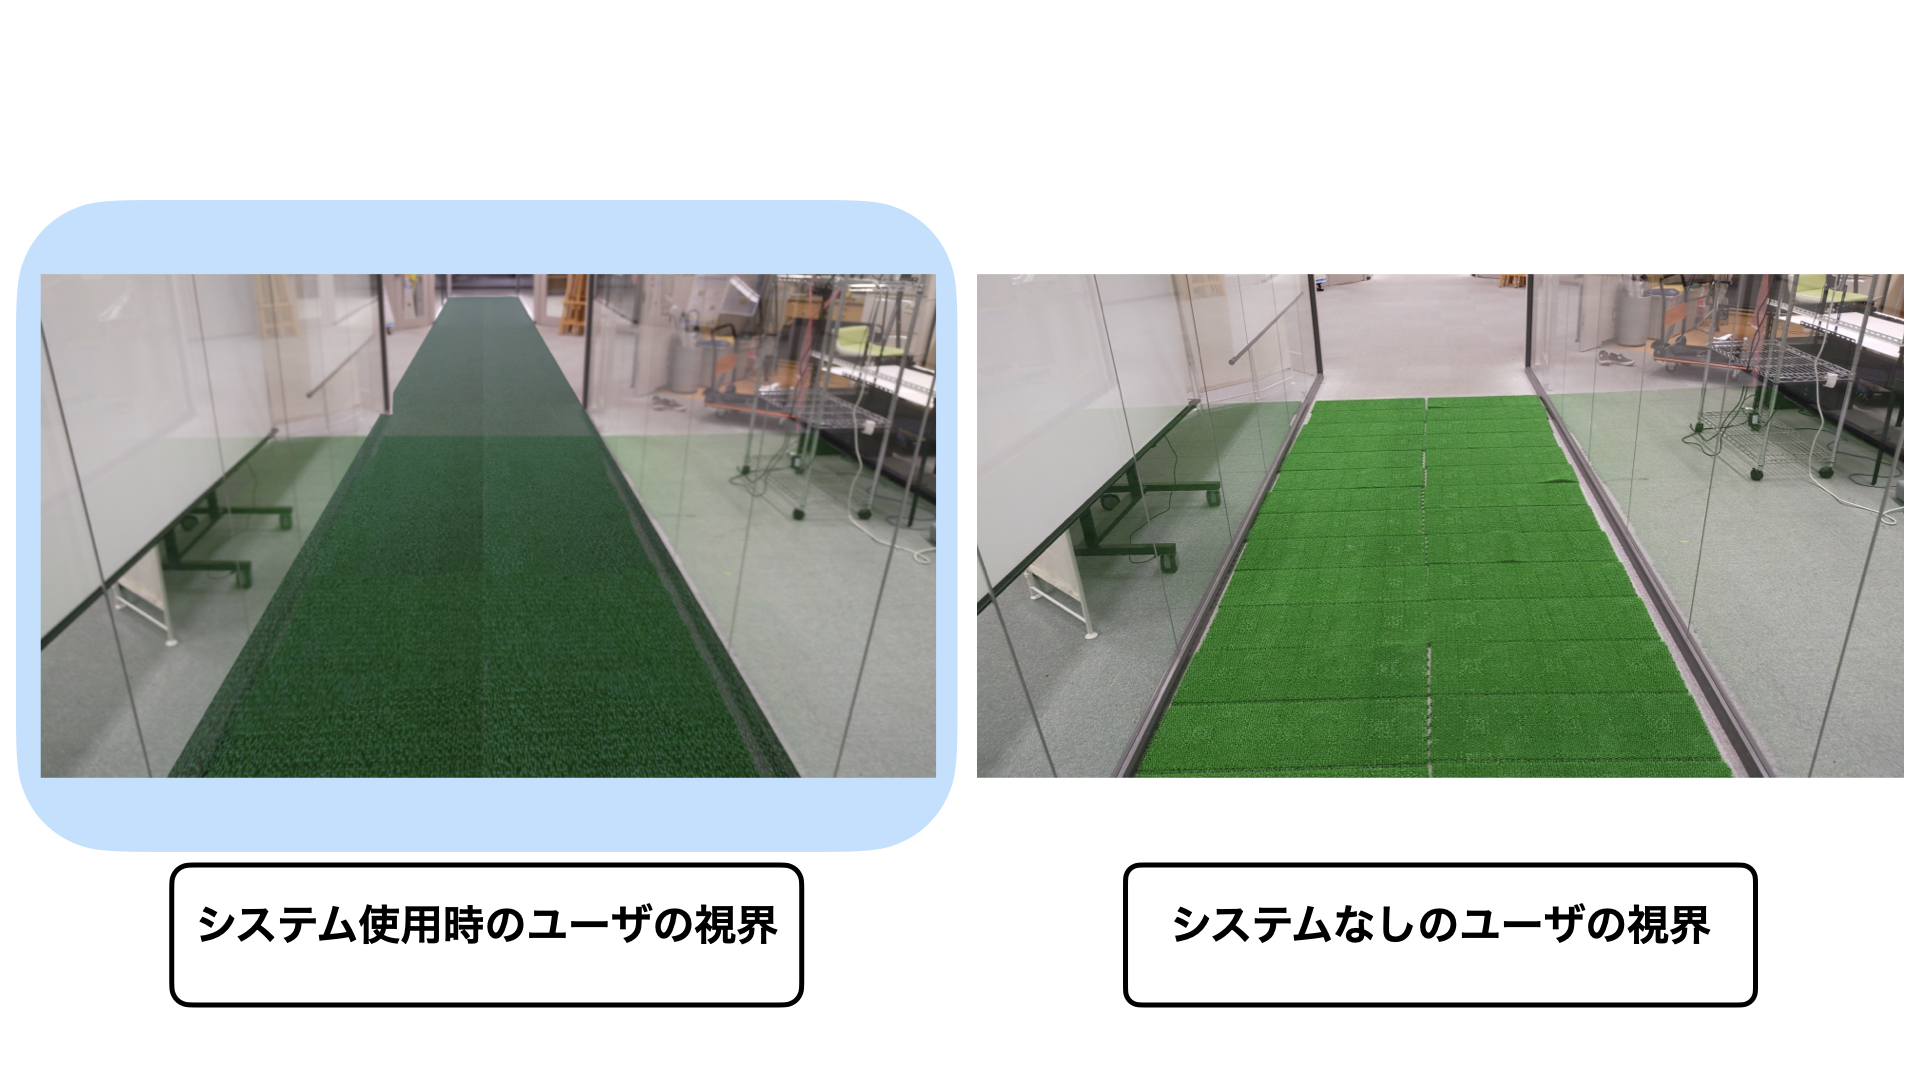
\includegraphics[width=1\linewidth]{fig/proto.001.jpeg}
    }
    \caption{プロトタイプ}
    \label{fig:puroto}
\end{figure}
図\ref{fig:puroto}に本システムのプロトタイプを示す.
プロトタイプでは上記の芝のリアルテクスチャをバーチャル床にアタッチし,床にアニメーション重畳表示を行なった.
バーチャル床はユーザの約20m前からこちらに向かうように動いてくる.
%------------------------------------------------------------------
\section{実験方法}

本稿では芝生道にて,芝生を模したバーチャル床を表示した場合,芝生を模していないバーチャル床を表示した場合を比べてユーザの歩行速度制御に優位性が出るか否かの調査を行う.
実験環境を図\ref{fig:kokaton}に示す.被験者は頭にはARグラスのHololens2を,体にはスマートフォンを揺れないように固定して装着してもらう.
実験手順を以下に示す.また、以下の手順をそれぞれ6回ずつ行なってもらい平均をとり,平均の値を評価では用いる.
\begin{enumerate}
    \item システムを使用していない状態のHololens2をつけてもらい,指定した道を指定距離歩いてもらう.
    \item 本システム(リアルテクスチャ or Nonリアルテクスチャ)を使用して歩いてもらう
    \item 手順2とは違うバージョンを使用して歩いてもらう
\end{enumerate}



 \section{評価方法}
 
 \subsection{感性評価}
 感性評価では,
The Simulator Sickness Questionnaire(SSQ)を用いたアンケートと,
5段階のリッカート尺度を用いたリアルテクスチャについてのアンケートを答えてもらい評価する.
 
 
 
 \begin{figure}[t]
    \centering
    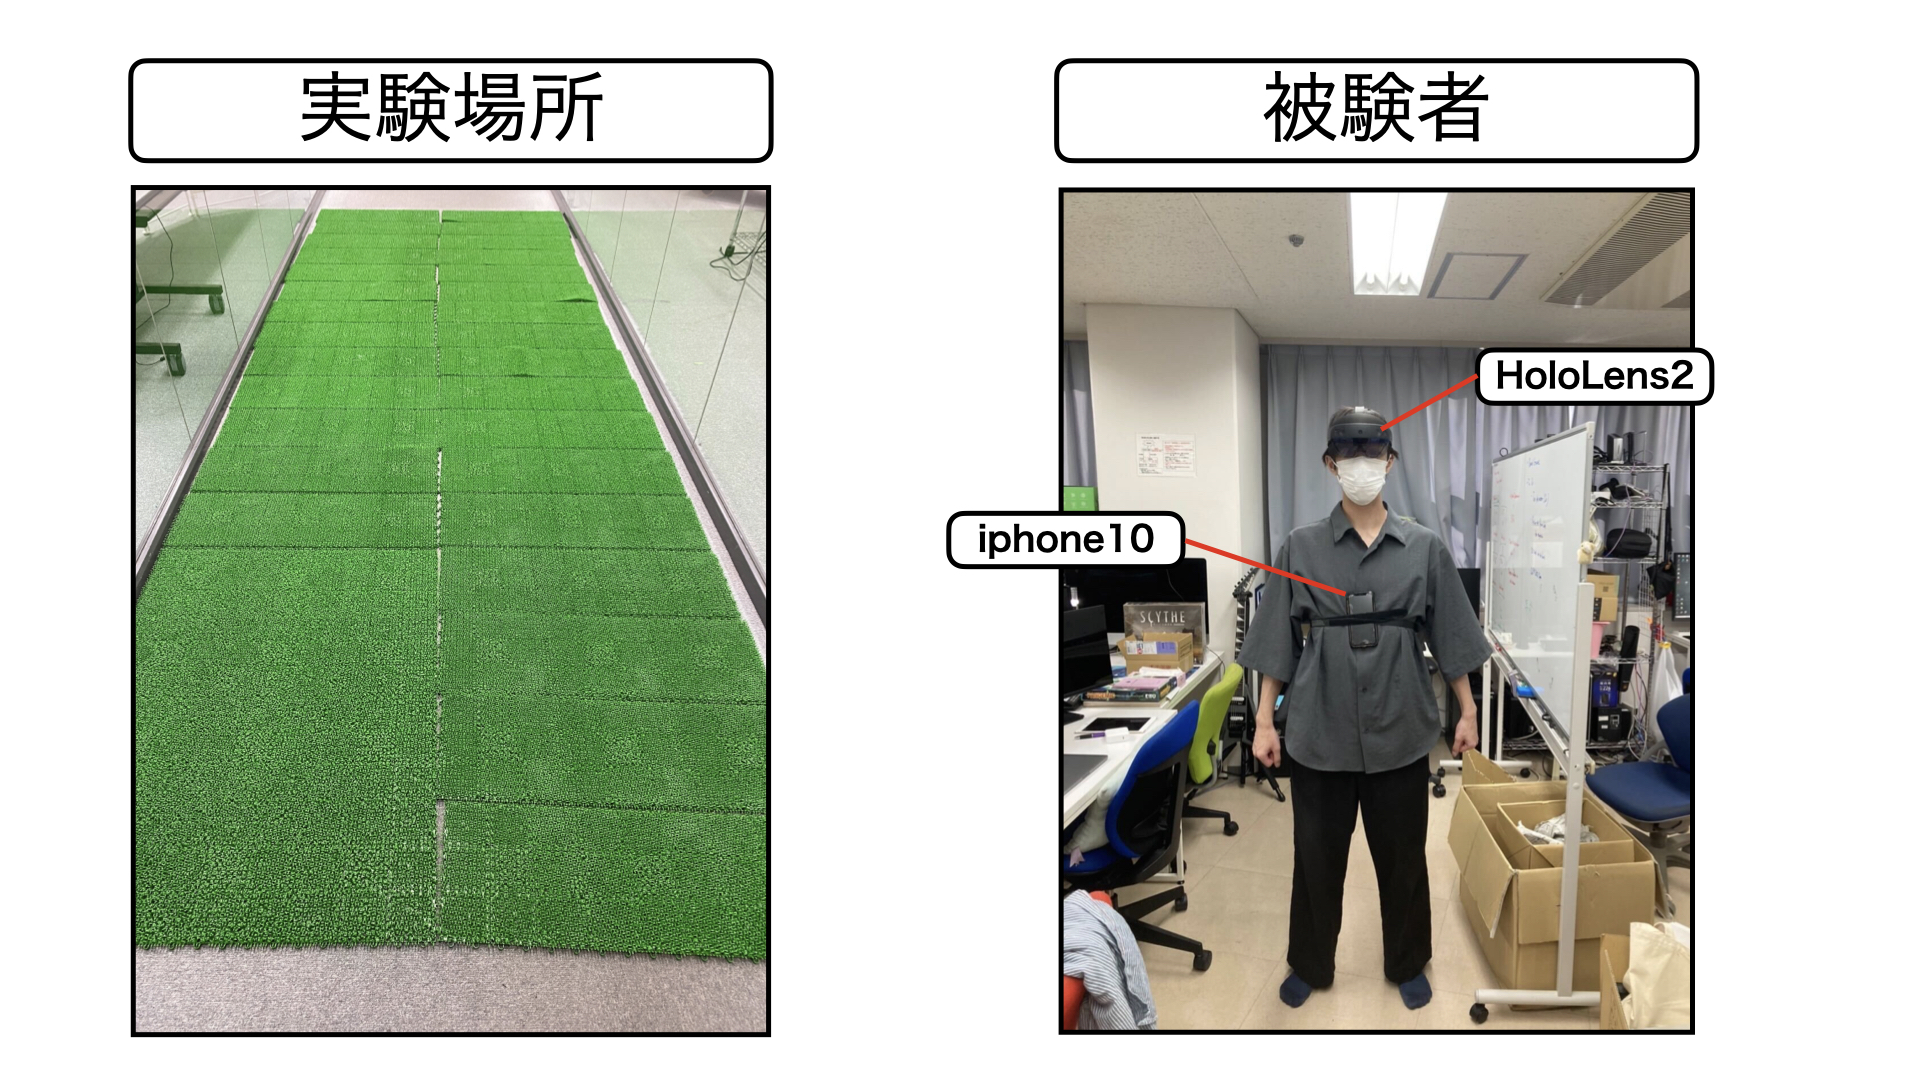
\includegraphics[width=0.8\linewidth]{fig/enviroment.jpeg}
    \caption{実験環境}
    \label{fig:kokaton}
\end{figure}

\subsection{定量評価}
 定量評価では,被験者の体に装着されたスマートフォンの加速度センサーを用いて,
 被験者の歩行速度は変化するのかを評価する.
評価する際s対応のある2標本t検定を用いて,以下の組み合わせで有位性を確認し評価を行う
\begin{itemize}
    \item システム無し・システム有り(リアルテクスチャ)
    \item システム無し・システム有り(Nonリアルテクスチャ1)
    \item システム無し・システム有り(Nonリアルテクスチャ2)
    \item システム無し・システム有り(Nonリアルテクスチャ3)
\end{itemize}
%------------------------------------------------------------------
\section{まとめ}
本研究では,地表面近似テクスチャーのアニメーション重畳表示よる歩行速度制御システムを提案した.
今後の課題として,Nonリアルテクスチャの選定,本システムを用いた実験が挙げられる.
また,実験結果からバーチャル床のテクスチャや挙動の改善を行う.
%------------------------------------------------------------------
\bibliographystyle{junsrt}
\bibliography{ref}
\end{document}
